\chapter{Pré-requis}
\section{Énoncé du sujet}
La génération automatique de terrains virtuels est un problème sur lequel planchent souvent les graphistes et les game designers, car pouvoir créer un monde virtuel persistant est une brique de base à de nombreuses applications. Mais, même si le sujet a été maintes fois traité, il reste un problème difficile non seulement techniquement à cause de la masse de calculs que cela représente mais aussi parce que le rendu final du paysage doit paraître un tant soit peu réaliste aux yeux des utilisateurs.\\

Le but de ce projet est de créer une bibliothèque permettant la création de terrains virtuels à partir de méthodes fractales et de créer un logiciel minimal de visualisation de ces terrains.\\

\section{Création d'un terrain}
La création d'un terrain, telle que nous la concevons, repose sur une série de 4 étapes que nous allons maintenant décrire :

\subsection{Mettre en place la grille}
Pour commencer, nous devrons mettre en place une grille à deux dimensions triangulaire ou carrée. Cette grille représentera le découpage du terrain. Le résultat final sera fonction de la grille de départ.

\subsection{Créer une carte d'élévations}
Une carte d'élévation (heightmap en anglais) est une matrice bi-dimentionnelle qui permet de décrire les hauteurs du terrain. Chaque entrée de la matrice stocke un nombre correspondant au taux d'élévation d'une intersection de la grille, 0 étant l'élévation minimale et 1 l'élévation maximale.
Cette matrice peut \^etre convertie en image en niveaux de gris (noir pour les creux, blanc pour les pics).\\
La figure~\ref{fig:heightmap} présente un exemple avec une grille carrée (attention, ici, des entiers sont utilisés alors que notre projet considèrera des flottants) :
\begin{figure}[h]
  \centering
  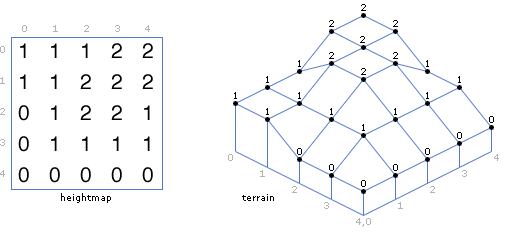
\includegraphics[scale = 0.55]{resources/heightmap_carre.png}
  \caption{Application de la heightmap à la grille}
  \label{fig:heightmap}
\end{figure}

\subsection{Créer une carte de coloration}
Il est ensuite possible d'ajouter des couleurs au terrain. Sur ce point, l'algorithme que nous utiliserons consistera à colorer les intersections de la grille en fonction des hauteurs données par la carte d'élévation.

\subsection{Raffiner le terrain}
Ici, le terrain est créé mais il est néanmoins possible d'en améliorer le réalisme. Nous passerons donc par une étape de raffinement qui consiste à appliquer, sur les hauteurs, des algorithmes faisant apparaitre des modifications locales, par exemple, des traces d'errosion.

\section{Visualisation d'un terrain}

\subsection{Exporter le terrain sous différents formats}
Il n'existe pas de format de fichiers standard commun à tous les visualisateurs. Un étape de traitement est donc nécessaire avant la visualisation. Celle-ci a pour but de rendre le terrain compatible avec le visualisateur utilisé. Il s'agit donc d'un export des données.

\subsection{Visualisation}
Cette dernière étape consiste à afficher le modèle en 3 dimentions \textit{via} un visualisateur.

 %% Mettre un schéma pour le pipeline


%Pour éviter la numérotation du sommaire
\thispagestyle{empty}
